%%
%% 2019 07 04 Ph. G. Freimann
%% 2020 Systematik verbessert
%%

\section{Lineare Funktionen}\index{Funktion!lineare}
\index{affin-lineare Funktionen}\label{lineare_funktionen}
\sectuntertitel{$f: \mathbb{R} \rightarrow \mathbb{R}$}
%%%%%%%%%%%%%%%%%%%%%%%%%%%%%%%%%%%%%%%%%%%%%%%%%%%%%%%%%%%%%%%%%%%%%%%%%%%%%%%%%
\subsection*{Lernziele}

\begin{itemize}
\item Begriff «Lineare Funktion»
\item Darstellungen (Wertetabelle, Funktionsgleichung, Graph)
\item Charakteristische Punkte\index{Punkt!charakteristischer}
  \begin{itemize}
  \item
    y-Achsenabschnitt (Ordinatenabschnitt)
  \item Nullstelle
  \end{itemize}
\item Steigung
\TALS{\item Taschenrechner: Darstellung von Graphen}
\end{itemize}

%%Theorie:
%%\TALS{(\cite{frommenwiler17alg} S.170 (Kap. 3.3))}
%%\GESO{(\cite{marthaler21alg}       S.237 (Kap. 14))}


\GESO{\matheNinjaLink{Lineare Funktionen}{https://olat.bbw.ch/auth/RepositoryEntry/572162163/CourseNode/108030887418864}}
\TALS{\matheNinjaLink{Lineare Funktionen}{https://olat.bbw.ch/auth/RepositoryEntry/572162090/CourseNode/108030908044855}}

\TadBMTA{237}{14}

\newpage

\subsection{Einstiegsbeispiel Taxiunternehmen}
Taxiunternehmen «A» hat eine Grundgebühr von CHF 10.- und kostet
danach CHF 0.60 pro gefahrenen Kilometer.

Taxiunternehmen «B» hat eine Grundgebühr von CHF 6.- und kostet
danach CHF 0.90 pro gefahrenen Kilometer.

Ab bzw. bis wo lohnt sich das Unternehmen «A» bzw. «B»?

  Zeichnen Sie ein Koordinatensystem. $x$-Achse = km; $y$-Achse = CHF.
  (Einteilung je ca. 20 Einheiten im 1. Quadranten.

\TRAINER{%%
    \bbwCenterGraphic{14cm}{allg/funktionen/img/Taxiunternehmen.png}

  Ablesen bei ca. 13-14 km.

  Rechnerisch:

  $$A(x): 10\text{[CHF]}
  +x\text{[km]}\cdot{} 0.60 \left[\frac{\text{CHF}}{\text{km}}\right] $$
  $$B(x): 6 +x \cdot{} 0.90$$
  Gleichstand bei:
  $$A(x) = B(x)$$
  $$10+0.6x = 6+0.9x$$
  Lösung:
  $$x = 13.\overline{3} \text{km}$$
}%% END TRAINER
\noTRAINER{%
    \bbwCenterGraphic{14cm}{allg/funktionen/img/LeerFuerTaxi.png}%
}%% end noTRAINER
\newpage
%%%%%%%%%%%%%%%%%%%%%%%%%%%%%%%%%%%%%%%%%%%%

\subsection{Taschenrechner}\index{Taschenrechner!Funktionen}

\GESO{
  Mit der ``TABLE''-Funktion auf Ihrem Taschenrechner lassen sich Wertetabellen ganz einfach erstellen.
  Füllen Sie eine Wertetabelle zur Funktion $f: y=\frac{3}{4}x  - 1.5$ aus und zeichnen Sie die Gerade in ein rechtwinkliges Koordinatensystem:

  \begin{tabular}{l|c|c|c|c|c|c|c}
    $x$ & -2 & -1 & 0 & 1 & 2 & 3 \\
    $y$ & \LoesungsRaumKurz{-3}   & \LoesungsRaumKurz{-2.25}   & \LoesungsRaumKurz{-1.5}  & \LoesungsRaumKurz{-0.75}  & \LoesungsRaumKurz{0}  &  \LoesungsRaumKurz{0.75} \\
  \end{tabular}


  \bbwGraph{-4}{4}{-4}{2}{
    \TRAINER{\bbwFunc{0.75*\x - 1.5}{-2.5:3.5}}
  }%% END bbw Graph
  %%\noTRAINER{\bbwGraph{-4}{4}{-4}{2}{}}
  %%\TRAINER{\bbwFunction{-4}{4}{-4}{2}{0.75*\x - 1.5}{-2.5:3.5}}  
}%% END GESO

\TALS{
  Erstellen Sie einen Graphen und definieren Sie die Funktion $f1$ wie
  folgt:

  $$f1(x) : = \frac{3}{4}x - 1.5$$

  Mit CTRL-T (Tabelle mit geteiltem
  Bildschirm) erscheint sofort auch die Wertetabelle.

  \begin{tabular}{l|c|c|c|c|c|c|c}
    $x$ & -2 & -1 & 0 & 1 & 2 & 3 \\
    $y$ & \LoesungsRaumKurz{-3}   & \LoesungsRaumKurz{-2.25}   & \LoesungsRaumKurz{-1.5}  & \LoesungsRaumKurz{-0.75}  & \LoesungsRaumKurz{0}  &  \LoesungsRaumKurz{0.75} \\
  \end{tabular}

  \bbwGraph{-4}{4}{-4}{2}{
    \TRAINER{\bbwFunc{0.75*\x - 1.5}{-2.5:3.5}}
  }%% END bbw Graph

}%% END TALS

\newpage%%

\subsection{Definition der linearen Funktion}\index{Lineare Funktion!Definition}

\begin{definition}{Lineare Funktion}{}
  Eine Funktion $f: x\mapsto f(x)$ von $\mathbb{R}$ nach $\mathbb{R}$ heißt
\textbf{linear}\index{lineare Funktion}, wenn sie in der Grundform
$$f(x) = y=a\cdot{}x + b$$
mit $a$ und $b$ in $\mathbb{R}$ dargestellt werden kann.
\end{definition}


Beispiele:

\vspace{3mm}
\hrule
\vspace{3mm}

$$f(x) = y = \LoesungsRaumLang{4x + 1.5}$$
(Hier ist $a=\LoesungsRaum{4}$ und $b=\LoesungsRaum{1.5}$.)

\vspace{3mm}
\hrule
\vspace{3mm}

$$f(x) = y = \LoesungsRaumLang{-x}$$
(Hier ist $a=\LoesungsRaum{-1}$ und $b=\LoesungsRaum{0}$.)

Ist $b=0$, so sprechen wir auch von einer Proportionalität.

\vspace{3mm}
\hrule
\vspace{3mm}

$$f(x) = y = \LoesungsRaumLang{-0.6}$$
(Hier ist $a=\LoesungsRaum{0}$ und $b=\LoesungsRaum{-0.6}$.)

Ist $a=0$, so sprechen wir auch von der konstanten Funktion.

\vspace{3mm}
\hrule

\subsection*{Aufgaben}
%%\GESOAadBMTA{250}{6. a) b)}

\GESO{\olatLinkArbeitsblatt{Lineare
    Funktionen}{https://olat.bbw.ch/auth/RepositoryEntry/572162163/CourseNode/102901171745363}{1. Funktionen skizzieren}}
\TALS{\olatLinkArbeitsblatt{Lineare
    Funktionen}{https://olat.bbw.ch/auth/RepositoryEntry/572162090/CourseNode/106131926046623}{1. Funktionen skizzieren}}


\newpage%%


\subsection{Charakteristiken}
%%
%%\subsection{Charakteristische Punkte}\index{Punkte!charakteristische}\index{charakteristische Punkte}
Jede lineare\footnote{
  Die linearen Funktionen werden eingeteilt in die \textbf{Proportionalitäten} für $b=0$ und in die \textbf{affinen Abbildungen} für $b\ne{}0$.} Funktion schneidet irgendwo die beiden\footnote{Ausnahme: Konstante. Eine Konstante $y=b$ schneidet nur die $y$-Achse. Der Spezialfall $y=0$ \textbf{ist} die $x$-Achse.} Achsen. Zeichnen Sie die Funktion $f: y=\frac{1}{2}x  +3$ und notieren Sie die Punkte, wo die x- bzw. die y-Achse von unserer Geraden geschnitten wird:

\vspace{1cm}

Wertetabelle:


\begin{tabular}{c|p{2cm}|p{2cm}|p{2cm}|p{2cm}|p{2cm}|p{2cm}}
   x  & 0 & 1 & 2 & 4 & -4 & \TRAINER{-6}\\\hline
   y  & \TRAINER{3} & \TRAINER{3.5} & \TRAINER{4}& \TRAINER{5}&\TRAINER{1}&0\\%%
\end{tabular}


\TNT{4}{
  Die Nullstelle bei $y=0$ wird entweder abgelesen, oder berechnet,
  indem wir in der Funktionsgleichung $y=\frac12x+3$ den Funktionswert
  $y=0$ setzen:
  $$0=\frac12x+3 \Longrightarrow x_0=-6$$
}

\bbwGraph{-7}{7}{-2}{5}{\TRAINER{
    \bbwDot{-6,0}{red}{east}{N}
    \bbwDot{0,3}{orange}{west}{Y}
    \bbwFuncC{3+0.5*\x}{-6.5:3.5}{blue}
}}
\newpage

\subsubsection{$y$-Achsenabschnitt}\index{$y$-Achsenabschnitt}\index{Achsenabschnitt!y-}\index{Ordinatenabschnitt}
\begin{definition}{$y$-Achsenabschnitt}{}
  Der Parameter $b$ wird $y$-Achsenabschnitt
(oder Ordinatenabschnitt\index{Ordinatenabschnitt}\footnote{Die
    $y$-Koordinate eines Punktes wird auch
    \textbf{Ordinate}\index{Ordinate} und die $x$-Koordinate wird auch
    \textbf{Abszisse}\index{Abszisse}  genannt.}) genannt.
  
Dieser gibt an, in welcher «Höhe» die Gerade die y-Achse schneidet.
\end{definition}

Wir erhalten den $y$-Achsenabschnitt, indem wir das Funktionsargument $x$
gleich Null (0) setzen: $x=0$.

Somit wird
$$y=ax+b$$
$$y=a\cdot{}0+b$$
$$y=b$$
Was uns zeigt, dass der  Punkt $P=(0|b)$ der Geraden immer auf der $y$-Achse liegt.

\subsection*{Aufgaben}
%%\GESOAadBMTA{250}{6. a) b)}

\GESO{\olatLinkArbeitsblatt{Lineare
    Funktionen}{https://olat.bbw.ch/auth/RepositoryEntry/572162163/CourseNode/102901171745363}{2. $y$-Achsenabschnitt}}
\TALS{\olatLinkArbeitsblatt{Lineare
    Funktionen}{https://olat.bbw.ch/auth/RepositoryEntry/572162090/CourseNode/106131926046623}{2. $y$-Achsenabschnitt}}




\newpage


\subsubsection{Steigung}\index{Steigung|textbf}
  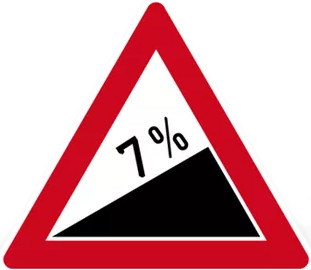
\includegraphics[width=4.5cm]{tals/trig1/img/starkeSteigung.jpg}

Der Parameter $a$ wird Steigung der Geraden genannt. Dies entspricht
dem $y$-Anstieg\footnote{Bei negativem $a$ sprechen wir von «Gefälle»,
  Abstieg, Neigung, Senkung, ...} der Geraden pro Einheit in $x$-Richtung ($e_x$):


%% Steigungsgraph: Eins nach rechts -> a noch oben (oder -a nach unten)
\bbwGraph{-4}{4}{-3}{4}{
	\draw[thick] (-4,-2.5) -- (4, 3.5);
	\draw[thick,color=blue] (1, 1.25) -- (2  , 1.25);
	\draw[thick,color=blue] (1, 1.25) -- (1.5, 1.25) node[anchor=north]{${\color{blue}1}$};
	\draw[thick,color=red ] (2, 1.25) -- (2, 2   );
	\draw[thick,color=red ] (2, 1.25) -- (2, 1.625   ) node[anchor=west ]{${\color{red}a}$ };
}

\newpage

Die Steigung $a$ kann aus \textbf{jedem} Steigungsdreieck berechnet werden,
wozu einfach zwei Punkte auf der Geraden zu verwenden sind:

%% Steigungsgraph: Eins nach rechts -> a noch oben (oder -a nach unten)
\bbwGraph{-4}{4}{-3}{4}{
	\draw[thick] (-4,-11/5) -- (4, 13/5);
	\draw[thick,color=blue] (-2, -1) -- (3,-1);
	\draw[thick,color=blue] (1, -1.1) node[anchor=north]{${\color{blue}H}$};
  
	\draw[thick,color=red] (3, -1) -- (3,2);
	\draw[thick,color=red] (3, 1.1) node[anchor=west]{${\color{red}V}$};

  \bbwDot{-2,-1}{black}{north}{}
  \bbwDot{3,2}{black}{north}{}
  \bbwDot{3,-1}{black}{north}{}
}


Steigt die Gerade in $x$-Richtung an, so ist ${\color{blue}a}$ positiv
(${\color{blue}a>0}$) {\color{blue} «Steigung»};\index{Steigung}
fällt die Gerade in $x$-Richtung ab, so ist ${\color{red}a}$ negativ
(${\color{red}a<0}$) {\color{red} «Gefälle»}.\index{Gefälle}

%% Steigungsgraph: Eins nach rechts -> a noch oben (oder -a nach unten)
\bbwGraph{-4}{4}{-3}{4}{
	\draw[thick,color=blue] (-4, -1) -- (4  , 3);
	\draw[thick,color=blue] (4, 3) node[anchor=north]{${\color{blue}+}$};
	\draw[thick,color=red ] (-3.5, 2) -> (4, -2);
	\draw[thick,color=red ] (4, -2) node[anchor=west ]{${\color{red}-}$ };
}
\newpage

\begin{rezept}{Finden der Geradensteigung}{}
Die Steigung $a$ ist:
$$a=\frac{{\color{red}V}}{{\color{blue}H}}$$
«Vau durch Haa, das gibt das Ahh!»
\end{rezept}

\subsubsection*{Herleitung (optional)}

\bbwCenterGraphic{10cm}{allg/funktionen/img/Steigungsdreieck.png}

\TNTeop{

 $$\frac{V}H = \frac{\Delta y}{\Delta x} = \frac{y_2-y_1}{x_2-x_1} =
  \frac{f(x_1) - f(x_2)}{x_2-x_1}$$

  $$= \frac{(a\cdot{}x_2 + b) - (a\cdot{}x_1 +b)}{(x_2-x_1)}$$
  $$= \frac{a\cdot{}x_2 + b - a\cdot{}x_1 -b}{(x_2-x_1)}$$
  $$= \frac{a\cdot{}x_2 - a\cdot{}x_1 }{(x_2-x_1)}$$
  $$= \frac{a\cdot{}(x_2 - x_1 )}{(x_2-x_1)}$$
  $$= a$$
}%% END TNT eop

%%%%%%%%%%%%%%%%%%%%%%%%%%%%%%%%%%%%%%%%%
\newpage


\subsection*{Aufgaben}
%%\GESOAadBMTA{250}{6. a) b)}

\GESO{\olatLinkArbeitsblatt{Lineare
    Funktionen}{https://olat.bbw.ch/auth/RepositoryEntry/572162163/CourseNode/102901171745363}{3. Steigung}}
\TALS{\olatLinkArbeitsblatt{Lineare
    Funktionen}{https://olat.bbw.ch/auth/RepositoryEntry/572162090/CourseNode/106131926046623}{3. Steigung}}
\newpage

\subsubsection{Nullstelle}\index{Nullstelle}
Eine steigende oder fallende lineare Funktion schneidet die $x$-Achse
in einem Punkt. Dieser Punkt wird \textbf{Nullstelle} genannt.

In der anfänglich untersuchten Funktion $f(x) = \frac12x+3$ schneidet
der Graph die $x$-Achse bei $-6$. 

\begin{definition}{Nullstelle}{}
  Eine \textbf{Nullstelle} $x_0$ gibt an, an welcher Stelle der Funktionsgraph die $x$-Achse schneidet.
\end{definition}


Die Nullstelle einer linearen Funktion in ihrer Grundform ist die Lösung der entsprechenden linearen Gleichung (mit
$y$=0) in ihrer Grundform. Nämlich:

\hrule

a) Lineare \textbf{Gleichung} $$ax+b=0$$

Gesucht \textbf{Lösung} $x$:

\TRAINER{$$ax+b=0 | -b$$}\noTRAINER{\mmPapier{1.2}}
\vspace{1mm}
\TRAINER{$$ax=-b | :a$$}\noTRAINER{\mmPapier{1.2}}

$$\lx = \TRAINER{\left\{\frac{-b}{a}\right\}}  $$

\hrule

b) Lineare \textbf{Funktion}/ $$f: y=ax+b$$

Gesucht \textbf{Nullstelle} $x_0$ bei $y_0=0$. Die Gerade schneidet
die $x$-Achse in der Nullstelle $x_0$ der Geraden.

\begin{gesetz}{Nullstelle}{}
  Die Nullstelle $x_0$ einer linearen Funktion berechnet sich wie folgt:
  
$$x_0 = \frac{-b}{a}$$
\end{gesetz}

Somit ist der
Schnittpunkt wie folgt gegeben:

$$N = (x_0|y_0) = (x_0|0) =\left( \frac{-b}{a}\,\, \bigg|\,\, 0 \right) $$
\newpage

\subsection*{Aufgaben}

\GESO{\olatLinkArbeitsblatt{Lineare Funktionen}{https://olat.bbw.ch/auth/RepositoryEntry/572162163/CourseNode/102901171745363}{4.1 und 4.2}}
\TALS{\olatLinkArbeitsblatt{Lineare Funktionen}{https://olat.bbw.ch/auth/RepositoryEntry/572162090/CourseNode/106131926046623}{4.1 und 4.2}}


\GESO{\olatLinkArbeitsblatt{Lineare Funktionen}{https://olat.bbw.ch/auth/RepositoryEntry/572162163/CourseNode/102901171745363}{4.3 - 4. 7}}
\TALS{\olatLinkArbeitsblatt{Lineare Funktionen}{https://olat.bbw.ch/auth/RepositoryEntry/572162090/CourseNode/106131926046623}{4.3 - 4.7}}
%%\AadBMTA{251ff}{10., 23. a) c) und optional 20. (Alkohol im Blut)}
\newpage

\subsection{Referenzaufgaben}\index{Lineare
  Funktion!Referenzaufgaben}\index{Referenzaufgaben zu linearen Funktionen}

\GESO{\subsubsection{Schnittpunkt zwischen zwei Geraden}

Wo schneiden sich die beiden folgenden Geraden $f$ und $g$?

$f: y=3x - 1$

$g: y=-\frac14x +2$

Bringen Sie die beiden Geraden je in die Grundform einer linearen
Gleichung mit zwei Variablen:

\gleichungZZ{-3x + y}{-1}{\frac{1}{4}x + y}{2}

Nun können Sie dieses Gleichungssystem einfach mit
der \textbf{SYS-SOLV}-Funktion Ihres Taschenrechners lösen.

\vspace{5mm}

\noTRAINER{\mmPapier{2.4}}
\TRAINER{$x=\frac{12}{13} y= \frac{23}{13}$}

\vspace{5mm}

\textbf{Alternative}

Eine weitere Möglichkeit ist es die beiden Funktionsterme gleich mit
der \texttt{num-solv}-Funktion des Taschenrechners gleichzusetzen:

\tiprobutton{2nd}\tiprobutton{sin_num-solv}: $3x-1 = -\frac14x+2$

Sie erhalten aber so nur den $x$-Wert des Schnittpunktes und müssen
den $y$-Wert durch Einsetzen danach noch bestimmen.

\newpage

\subsection*{Aufgaben}
\GESO{\olatLinkArbeitsblatt{Lineare
Funtkionen}{https://olat.bbw.ch/auth/RepositoryEntry/572162163/CourseNode/102901171745363}{5. Schnittpunkte}}

\newpage
}
\TALS{\subsubsection{Schnittpunkt zwischen zwei Geraden}

Wo schneiden sich die Geraden $f: y=3x - 1$ und $g: y=-\frac14x + 2$?

Zeichnen Sie zunächst eine Skizze:

\bbwGraph{-4}{4}{-4}{5}{
\bbwFunc{3*\x - 1}{-1.5:2}{blue}
\bbwFunc{-\x/4 +2}{-1.5:2}{blue}
}

Gibt es eine Möglichkeit, den Schnittpunkt rechnerisch zu bestimmen?

\TNTeop{
$$f(x_s)=y=g(x_s)$$

$$3x-1 = -\frac14x + 2$$
$$\frac{13}4x = 3$$

$x=\frac{12}{13} y= 3\cdot{}\frac{12}{13} - 1 =\frac{36}{13}-\frac{13}{13} =\frac{23}{13}$

$$S = \left(\frac{12}{13}\middle|\frac{23}{13}\right)$$
}%% END TNTeop


\newpage

\TALS{%%

\subsubsection{Schnittpunkt zweier Funktionen mit dem Taschenrechner}

Nehmen wir zur Abwechslung zwei andere Funktionen, von denen wir den
Schnittpunkt ihrer Graphen bestimmen wollen:

$$f(x) :=  \frac{x}{4}  - 2$$
$$g(x) := -\frac{3}{2}x + 5$$

\[
%%\begin{equation}%% but equation makes a number (1)
    gls:= \left\{\begin{array}{@{}lr@{}}
        f(xs) = ys\\
        g(xs) = ys
        \end{array}\right.
\]
%%\end{equation}

  $$solve(gls,\{xs, ys\})$$
  \TRAINER{Lösung S(4|-1)}
}%%
}
\newpage




\paragraph{Die zwei Parallelen} (Christian Morgenstern)
\begin{verse}
Es gingen zwei Parallelen\\
ins Endlose hinaus,\\
zwei kerzengerade Seelen\\
und aus solidem Haus.

Sie wollten sich nicht schneiden\\
bis an ihr seliges Grab:\\
Das war nun einmal der beiden\\
geheimer Stolz und Stab.

Doch als sie zehn Lichtjahre\\
gewandert neben sich hin,\\
da wards dem einsamen Paare\\
nicht irdisch mehr zu Sinn.

War'n sie noch Parallelen?\\
Sie wußtens selber nicht, ---\\
sie flossen nur wie zwei Seelen\\
zusammen durch ewiges Licht.

Das ewige Licht durchdrang sie,\\
da wurden sie eins in ihm;\\
die Ewigkeit verschlang sie\\
als wie zwei Seraphim.
\end{verse}
\newpage

\subsubsection{\TALS{Senkrechte und
  }Parallele}\index{Parallele}\TALS{\index{Senkrechte}}\index{Parallele}

Skizzieren Sie $f: y=\frac{1}{4}x +3$ und $g:
y=\frac{1}{4}x -1$. Was fällt Ihnen auf?

\bbwGraph{-1}{6}{-2}{5}{}


\textbf{Parallele}:\\

\begin{center}
\begin{tabular}{c|c}
  Gerade     & Parallele   \\
  \hline
  $y=ax+b_1$ & $y=ax+b_2$ \\
\end{tabular}
\end{center}


\TALS{
\newpage
 Zeichnen Sie eine Senkrechte zur folgenden Geraden:

\bbwGraph{-1}{6}{-2}{4}{
  \bbwLine{-1,-1.25}{6,0.5}{green}
  \bbwDot{0,-1}{blue}{east}{}
  \bbwDot{4,0}{blue}{north}{}
}%% END bbwGraph

\textbf{Senkrechte (Lot)\index{Senkrechte}\index{Lot}}

\begin{center}
\begin{tabular}{c|c}
  Gerade     & Senkrechte \\
  \hline
  $y=ax+b_1$ & $y=-\frac{1}{a}x + b_3$\\
\end{tabular}
\end{center}

Da es beliebig viele Senkrechte und Parallele zu einer gegebenen
Geraden gibt, kann nur auf die Steigung eine Aussage gemacht
werden. Sowohl $b_2$, wie auch $b_3$ können erst ermittelt werden,
wenn weitere Angaben (wie \zB{} ein weiterer Punkt) vorhanden sind.

Beachten Sie, dass hier $a$ natürlich nicht Null (0) sein darf.
}

\GESO{
Da es beliebig viele Parallele zu einer gegebenen
Geraden gibt, kann nur auf die Steigung eine Aussage gemacht
werden. $b_2$ kann erst ermittelt werden,
wenn weitere Angaben (wie \zB{} ein weiterer Punkt) vorhanden sind.
}

\newpage


\subsection*{Aufgaben}
\GESO{\olatLinkArbeitsblatt{Lineare Funktionen}{https://olat.bbw.ch/auth/RepositoryEntry/572162163/CourseNode/102901171745363}{6. Parallele}}
\TALS{\olatLinkArbeitsblatt{Lineare Funktionen}{https://olat.bbw.ch/auth/RepositoryEntry/572162090/CourseNode/106131926046623}{6. Parallele}}
\newpage


\subsubsection{Ein Punkt ist gegeben}\index{Punkt auf Geraden}\index{Gerade!Punkt auf|textbf}
Bei vielen Anwendungen ist von der Geraden die Steigung $a$
\textbf{oder} der $y$-Ach\-sen\-ab\-schnitt $b$ gegeben, aber nicht
beides. Dabei ist meist ein Punkt $P$ (\zB $P=(7|4)$) gegeben, durch
den die Gerade laufen muss.

Gleich zwei Beispiele:

\begin{tabular}{p{8cm}|p{8cm}}\hline
  Steigung gegeben & $y$-Achsenabschnitt gegeben \\\hline
  $y$-Achsenabschnitt gesucht & Steigung gesucht \\\hline
  ${\color{orange}y}=3\cdot{}{\color{blue}x}+b$ & ${\color{orange}y}=a\cdot{}{\color{blue}x}+1.5$\\
  \hline
  Punkt $P=({\color{blue}7}|{\color{orange}4})$ gegeben & Punkt $P=({\color{blue}7}|{\color{orange}4})$ gegeben\\
  \hline
  einsetzen: & einsetzen: \\
  $\LoesungsRaumKurz{{\color{orange}4}} = 3\cdot{}\LoesungsRaumKurz{{\color{blue}7}} + b$ & $\LoesungsRaumKurz{{\color{orange}4}}=a\cdot{}\LoesungsRaumKurz{{\color{blue}7}} + 1.5$\\
  \hline
  lösen & lösen\\
  \end{tabular}


\TNT{6}{
\begin{tabular}{c|c}
$  4 =3\cdot 7 + b$ & $ 4           =7a +1.5$ \\
$  4 =21       + b$ & $ 2.5         =7a     $ \\
$-17 =           b$ & $ \frac{2.5}7 = a     $ \\
$b = -17          $ & $ a = \frac{5}{14} \approx 0.357    $ \\
$y = 3x-17        $ & $ y=\frac5{14}\cdot{x} + 1.5   $ \\
\end{tabular}
}

\begin{rezept}{Einsetzen}{}
Koordinaten des gegebenen Punktes in die
  Geradengleichung einsetzen, um $a$ bzw. $b$ zu finden!
\end{rezept}

\subsection*{Aufgaben}
\GESO{\olatLinkArbeitsblatt{Lineare
  Funktionen}{https://olat.bms-w.ch/auth/RepositoryEntry/6029794/CourseNode/102901171745363}{7.1
  und 7.2}}
\TALS{\olatLinkArbeitsblatt{Lineare
  Funktionen}{https://olat.bms-w.ch/auth/RepositoryEntry/6029786/CourseNode/106131926046623}{7.1
  und 7.2}}

%% obsolet, da Geradenbestimmung bereits gemacht. \GESOAadBMTA{255ff}{34. a) b) und 35.}

\newpage

%% 
\subsubsection{Gerade durch zwei gegebene Punkte}\index{Punkt auf Geraden}\index{Gerade!Punkt auf}
\TRAINER{\TALS{ev. Einstiegsaufgaben Frommenwiler: 606. a) c)}}

Seien die Punkte $P=(10|6)$ und $Q=(-5|3)$ gegeben.
Gesucht ist die Funktionsgleichung $f: y=ax+b$ (namentlich $a$ und $b$), sodass
der Graph der Funktion $f$ durch beide Punkte führt.


\textbf{Rezept I: Graphisch}\\

\vspace{1mm}

\TNTeop{%%
\raisebox{2cm}{\includegraphics[width=16cm]{allg/funktionen/img/GeradeDurchZweiPunkte.jpg}}}%% END TNT EOP 

\newpage

\textbf{Rezept II: Rechnerisch, algbraisch \GESO{(optional)}}\\

\vspace{1mm}

\begin{rezept}{}{}
Um die Funktionsgleichung $$y=ax+b$$ zu finden,
  werden die $x$- und $y$-Koordinaten der beiden Punkte in die Gleichung eingesetzt und die beiden Gleichungen werden nach $a$ und $b$ aufgelöst. 
\end{rezept}

a)

Das $a$ kann durch das «Steigungsdreieck» berechnet werden:

$$a = \frac{y_Q-y_P}{x_Q-x_p} = \LoesungsRaumLang{\frac{3 - 6}{(-5) - 10} = \frac{-3}{-15} = \frac{1}{5}}$$

b)

Setzen wir $a=\frac{1}{5}$ und einen der beiden Punkte (\zB $P=(10|6)$) in die
allgemeine Funktionsgleichung $y=ax+b$ ein, so erhalten wir

\TNT{2}{$$y=\frac15x+b$$
$$6=\frac15\cdot{}10 + b$$
$$b=4$$}

Die gesuchte Geradengleichung lautet also:

$$f: y=\LoesungsRaumLang{\frac{1}{5}\cdot{}x + 4}$$

\GESO{\newpage
\textbf{Rezept III: Mit dem Taschenrechner}
Wieder seien die beiden Punkte $P=(10|6)$ und $Q=(-5|3)$ gegeben.

Tippen Sie auf dem Taschenrechner \tiprobutton{data}, um mit der
Eingabe der beiden Punkte zu beginnen. Geben Sie in die
Spalte \texttt{L1} die $x$-Werte und in die Spalte \texttt{L2} die
$y$-Werte ein:

\begin{tabular}{c|c|}
 \texttt{L1}& \texttt{L2} \\\hline
 \noTRAINER{.....}\TRAINER{10}  & \noTRAINER{.....}\TRAINER{6}\\
 \noTRAINER{.....}\TRAINER{-5}  & \noTRAINER{.....}\TRAINER{3}
\end{tabular}

Wählen Sie mit \tiprobutton{2nd} \tiprobutton{data_stat-reg-distr}
unter \texttt{STAT-REG} die Nummer 4: «\texttt{LinReg} $ax+b$».
Lassen Sie die Werte auf den nächsten Seite so stehen wie sie sind:

xDATA: L1

yDATA: L2

Mittels \texttt{CALC} (\tiprobutton{enter}) erhalten Sie $a=0.2$ und $b=4$.

}%% END GESO

\TALS{\newpage}


\TALS{%%
Dies kann auch mit dem Taschenrechner gelöst werden; denn für alle Punkte $P$ auf $f$ gilt ja $P(x|y) = P(x|f(x))$:

$$f(x):=a\cdot{}x + b$$
\[
%%\begin{equation}%% but equation makes a number (1)
    gls:= \left\{\begin{array}{@{}lr@{}}
        f(10) = 6\\
        f(-5) = 3
        \end{array}\right.
\]
%%\end{equation}

  $$solve(gls,\{a, b\})$$
}%%

\subsection*{Aufgaben}

\AadBMTA{252ff}{13. a), 14. a), 15. a), 16. a), 18. a), 19., 25. a)}

\newpage%%

\newpage

\TALS{\subsubsection{Referenzaufgabe: Abstand}\index{Abstand!zwischen Punkt und Gerade}

Gegeben ist ein Punkt $P=(1|3.5)$ und eine Gerade $f: y=\frac{1}{4}x-1$. Gesucht ist der Abstand des Punktes $P$ zu $f$.

\newcommand{\vorgehensTitelchen}[1]{\textbf{\color{brown}#1
\\
}}

Wie ist der Abstand zwischen einem Punkt und einer Geraden wohl definiert?

\vorgehensTitelchen{1. Skizze}
\bbwGraph{-1}{6}{-2}{4}{
 \bbwDot{1,3.5}{blue}{west}{P}
      \bbwLine{-1,-1.25}{5,0.25}{green}
    \TRAINER{
    \bbwLine{0.875,4}{2.25,-1.5}{red}}
  }
  
Suchen Sie in obiger Skizze den Abstand und messen/schätzen Sie ihn.


\vorgehensTitelchen{2. Senkrechte ($g\perp f$)}

\TNT{1.2}{
  $g: y = ax + b$ mit $a = -4$ (negativer Kehrwert aus $f$). Ergo:
  $g: y = -4x + b$
}

\vorgehensTitelchen{3. $g$ durch $P$ ($P\in g$)}

\TNT{2.8}{Kernidee: Punkt in Funktionsgleichung einsetzen:

  $P=(1|3.5)$ in $y=-4x+b$ einsetzen: $3.5 = -4\cdot{} (1) + b$

  Daraus errechnen wir $b = 7.5$. Und es folgt
$$g: y= -4x+7.5$$}

\newcommand\mussgleich{\mathrel{\stackrel{\makebox[0pt]{\mbox{\normalfont{\tiny{!}}}}}{=}}}

\vorgehensTitelchen{4. Schnittpunkt S ($S := g\cap f$)}

\TNT{3.2}{Idee: Beide Funktionsterme gleichsetzen, denn $S(x_s|y_s)$ muss auf beiden Geraden liegen:
  $$g(x_s) = y_s = f(x_s)$$
  $$-4x_s + 7.5 \mussgleich{} \frac{1}{4}x_s - 1$$
  ausrechnen lassen
$\Rightarrow x_s = 2 \Rightarrow y_s= \frac14x-1 = \frac14\cdot{}2 - 1
  = \frac12; S=(2|-\frac12) $}
\noTRAINER{\newpage}

\vorgehensTitelchen{5. Abstand mit Pythagoras ($\left|\overline{PS}\right|$)}

\TNTeop{$P=(1|3.5), S(2|-0.5) \Rightarrow \sqrt{(2-1)^2 +
  (-0.5-3.5)^2}= \sqrt{17} \approx 4.123 $}
\newpage

\TALS{
\subsubsection{TI nSpire}
Wie sieht das mit dem CAS-fähigen Taschenrechner TI nSpire aus? Hier
ein Beispiel einer Geraden $f1: y=\frac{4}{3}x-2$ und dem Punkt
$P=(-1|5)$.

\leserluft{}

\bbwCenterGraphic{17cm}{allg/funktionen/img/AbstandGeradeZuPunkt.png}

\begin{bbwFillInTabular}{ll}
Funktionsgleichung & $f_2(x)=$\LoesungsRaumLang{$\frac{-3}{4}x + \frac{17}{4}$}\\
Schnittpunkt       & $S=(\LoesungsRaum{3} | \LoesungsRaum{2})$\\
Abstand            & $\overline{PS} = \LoesungsRaum{5}$
\end{bbwFillInTabular}


\subsection*{Aufgaben}
\AadBMTA{256}{35. a), 36. a), 37. a)}
\newpage
}%% END TALS

\newpage}

\GESO{
\subsection*{Vermischte Aufgaben zu linearen Funktionen}
\olatLinkGESOKompendium{3.2}{20ff}{3. bis 26.}
\newpage
}%% END GESO

\subsection{Lineare Gleichungen visualisieren\GESO{ (optional)}}\index{Gleichungen!visualisieren}\index{Visualisierung von Gleichungen}
Wir gehen von der linearen\footnote{Eine Gleichung, bzw. ein Term
  heißt «linear», wenn die Variable ($x$) nur in der ersten Potenz vorkommt.} Gleichung $$4x+3x -18 + 16x = 5$$ aus.

Bringen wir alle Summanden nach links, so erhalten wir folgende
Gleichung:

\TNT{2}{$$4x + 3x  -18 + 16x  - 5= 0$$}%% END TNT


Schreiben wir dies als Funktion in $x$, so können wir folgende
Funktion definieren:

$$f(x): x \mapsto y = \TRAINER{4x+3x-18+16x - 5}$$

Stellen wir diese Funktion nun graphisch dar, so ergibt sich folgendes
Bild:

\TRAINER{\raisebox{-1cm}{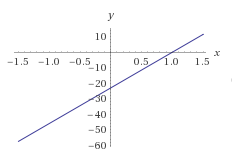
\includegraphics[width=7cm]{allg/funktionen/img/FunktionsplotAusGleichung.png}}}
\noTRAINER{\raisebox{-1cm}{\includegraphics[width=7cm]{allg/funktionen/img/KoordSystemFaktor20.png}}}


Die Lösung obiger Gleichung kann nun auf der $x$-Achse ungefähr bei $x=1.0$ abgelesen werden.
\newpage

\subsection*{Aufgaben}
%%\TALSAadBFWA{171ff}{601. a) b) c) e) f) 602. b) c) d) 603. b) c)
%% 604. 605. a) c) e) 606. a) c) 607. c) d) g) 608. a) 609. a) 610. a)
%% 611. a) 613. a) 616. c) 622. Flächen: 626. 628. und 629.}

\GESO{\olatLinkArbeitsblatt{Lineare Funktionen}{https://olat.bbw.ch/auth/RepositoryEntry/572162163/CourseNode/102901171745363}{7.}}
\TALS{\olatLinkArbeitsblatt{Lineare Funktionen}{https://olat.bbw.ch/auth/RepositoryEntry/572162090/CourseNode/106131926046623}{7.}}

\GESO{\olatLinkGESOKompendium{3.2}{25}{27.}}

\GESO{
  Alte Maturprüfungsaufgaben zu linearen Funktionen:
  
  \olatLinkArbeitsblatt{Alte Maturprüfungsaufgaben zu linearen Funktionen}{https://olat.bbw.ch/auth/RepositoryEntry/572162163/CourseNode/107461640594784}{05\_Lineare\_Funktionen\_alte\_Prüfungsaufgaben\_GESO.pdf}
  %%\newpage \subsection{Aus alten Maturaprüfungen}

\subsubsection{Serie 2017 Aufgabe 10}

Gegeben ist folgende Funktionsgleichung der Geraden $g$:

$$g: y = -3.75x + \frac{1}{4}$$

a) Bestimmen Sie die Schnittpunkte von $g$ mit den Koordinatenachsen.
Geben Sie die exakten Werte an.

\TNTeop{Schnittpunkt mit der $y$-Achse heißt $x=0$ also $y=-3.75\cdot{}0 + \frac{1}{4} = \frac{1}{4}$. Somit ist der Schnittpunkt mit der $y$-Achse $(0 | \frac{1}{4})$.

Schnittpunkt mit der $x$-Achse heißt $y=0$ also $0=-3.75\cdot{}x + \frac{1}{4}$. Gleichung Auf"|lösen: Auf beiden Seiten $- \frac{1}{4}$ ergibt

$$-\frac{1}{4} = -3.75 x$$
Nun beide Seiten dividieren durch $-\frac{1}{4}$ ergibt:

$$1 = 15x$$

Und somit ist $x=\frac{1}{15}$, und der gesuchte Punkt auf der $x$-Achse lautet $(\frac{1}{15} | 0)$.


}%% END eop

%%%%%%%%%%%%%%%%%%%%%%%%%%%%%%%%%%%%%%%

b) Nennen Sie zwei verschiedene Punkte $A(x_A | y_A)$ und $B(x_B | y_B)$, die
auf $g$ liegen und folgende Vorgabe erfüllen:

$x_A$, $y_A$, $x_B$ und $y_B$ müssen ganzzahlig sein. \TRAINER{\zB Wertetabelle im TR mit x= -10 step 1}

\TNTeop{
  \bbwGraph{-4}{4}{-13}{6}{
    \bbwFunc{-3.75*\x+0.25}{-2:3.5}
 \bbwDot{3,-11}{blue}{west}{B}
 \bbwDot{-1,4}{blue}{east}{A}
}%% END BBW Graph
}%% END TRAINER


%%%%%%%%%%%%%%%%%%%%%%%%%%%%%%%%%%%%%%%%%%%%%%%%%%%%%%%%%%%%%5

\subsubsection{2016 Aufgabe 7}

Carunternehmen A bietet folgenden Tarif an:
Pro Tag CHF 300.-- Grundtaxe und für jeden gefahrenen Kilometer CHF 1.50.

Bei Unternehmen B bezahlte eine Reisegruppe für Grund- und Kilometertaxe für einen
Tagesausflug von 600 km den Betrag von CHF 1320.--.

Eine andere Gruppe, die ebenfalls mit Unternehmen B fuhr, bezahlte mit demselben
Tarif für einen Tagesausflug von 750 km den Betrag von CHF 1590.-- .

a) Bestimmen Sie die Kostenfunktionen $y = f(x)$ für die Unternehmen A und B;
$x$ = Anzahl km gefahrene Strecke, $y$ = Anzahl CHF Gesamtkosten.

\TNT{5.6}{A: $y=1.5x + 300$

B: Steigungsdreieck: $a=\frac{1590 - 1320}{750-600} = \frac{270}{150} = 1.8$ daraus folgt $y = 1.8x + b$. Nun können wir die erste Reisegruppe einsetzen: $1320 = 1.8\cdot{}600 + b$ und somit ist $b= 240$. Die Funktionsgleichung lautet also

B: $y = 1.8x + 240$
\vspace{30mm}
}%% END TRAINER

b)  Bei welcher Fahrstrecke sind beide Firmen gleich teuer?
{\small Es müsste in der Aufgabenstellung wohl «Unternehmen» lauten; wird aber vorausgesetzt, dass verstanden wird, was gemeint ist.}

\TNTeop{
$y$ = Kosten gleichsetzen: $1.5x + 300 = 1.8x + 240$. Gleichung auf"|lösen: $60 = 0.3x$ und somit $x=200$. Ergo: Bei 200 km sind beide Unternehmen (=Firmen) gleich teuer.
}%% end TRAINER eop

%%%%%%%%%%%%%%%%%%%%%%%%%%%%%%%%%%%%%%%%%%%%%%%%%%%%%%%%%%%%%%%

c) 
Zwei weitere Firmen, C und D, haben folgende Kostenfunktion:

Firma C: $y = 1.8x + 250$ , Firma D: $y = 2.5x + 150$ ;

$x$ = Anzahl km gefahrene Strecke, $y$ = Anzahl CHF Gesamtkosten.

Eine Reisegruppe wählt für einen Tagesausflug von 300 km Länge Firma D, da diese
den ansprechenderen Internetauftritt hat. Um welchen Betrag wird diese Reise gegen-
über dem Angebot von Firma C teurer?

\TNTeop{300 km in beide Funktionsgleichungen als $x$-Wert eintragen: C kostet $1.8\cdot{}300 + 250 = 790$; D kostet $2.5\cdot{}300 + 150 = 900$. Somit kostet D CHF 110.-- mehr als C.

}%% end TRAINER

%%%%%%%%%%%%%%%%%%%%%%%%%%%%%%%%%%%%%%%%%%%%%%%%

\subsubsection{2018 Serie 1 Aufgabe 9}

Gegeben ist die Gerade $g$ mit der Funktionsgleichung $y = \frac{2}{3}x-4$.

a) Berechnen Sie den Schnittpunkt von $g$ mit der $x$-Achse.

\TNT{6}{Schnittpunkt mit der $x$-Achse heißt $y=0$. Somit $0 = \frac{2}{3}x - 4$ nach $x$ auf"|lösen:
$4=\frac{2}{3}x$ $\longrightarrow$ $6 = x$. Der Schnittpunkt ist folglich $(6|0)$.

  \vspace{60mm}
}%% end TRAINER

b) Welche der folgenden Punkte $A$, $B$, $C$ liegen \textit{oberhalb}, welche
\textit{unterhalb} und welche \textit{auf} der Geraden $g$?

$$A\left(5\middle|-\frac{3}{4}\right), B(2.1|-2.6), C(50|30)$$

\textbf{Antworten:}

\begin{tabular}{lcl}
$A$ liegt & \TRAINER{unterhalb}\noTRAINER{....................................................} & der Geraden $g$.\\
$B$ liegt & \TRAINER{auf}\noTRAINER{....................................................} & der Geraden $g$.\\
$C$ liegt & \TRAINER{oberhalb}\noTRAINER{....................................................} & der Geraden $g$.\\

 \end{tabular}

\TNTeop{Jeweils $x$ in die Gleichungen einsetzen und mit $y$ vergleichen.}%% End TNT

}%% end GESO


\newpage%%
